\documentclass[fleqn]{beamer}\usepackage[]{graphicx}\usepackage[]{color}
% maxwidth is the original width if it is less than linewidth
% otherwise use linewidth (to make sure the graphics do not exceed the margin)
\makeatletter
\def\maxwidth{ %
  \ifdim\Gin@nat@width>\linewidth
    \linewidth
  \else
    \Gin@nat@width
  \fi
}
\makeatother

\definecolor{fgcolor}{rgb}{0.345, 0.345, 0.345}
\makeatletter
\@ifundefined{AddToHook}{}{\AddToHook{package/xcolor/after}{\definecolor{fgcolor}{rgb}{0.345, 0.345, 0.345}}}
\makeatother
\newcommand{\hlnum}[1]{\textcolor[rgb]{0.686,0.059,0.569}{#1}}%
\newcommand{\hlstr}[1]{\textcolor[rgb]{0.192,0.494,0.8}{#1}}%
\newcommand{\hlcom}[1]{\textcolor[rgb]{0.678,0.584,0.686}{\textit{#1}}}%
\newcommand{\hlopt}[1]{\textcolor[rgb]{0,0,0}{#1}}%
\newcommand{\hlstd}[1]{\textcolor[rgb]{0.345,0.345,0.345}{#1}}%
\newcommand{\hlkwa}[1]{\textcolor[rgb]{0.161,0.373,0.58}{\textbf{#1}}}%
\newcommand{\hlkwb}[1]{\textcolor[rgb]{0.69,0.353,0.396}{#1}}%
\newcommand{\hlkwc}[1]{\textcolor[rgb]{0.333,0.667,0.333}{#1}}%
\newcommand{\hlkwd}[1]{\textcolor[rgb]{0.737,0.353,0.396}{\textbf{#1}}}%
\let\hlipl\hlkwb

\usepackage{framed}
\makeatletter
\newenvironment{kframe}{%
 \def\at@end@of@kframe{}%
 \ifinner\ifhmode%
  \def\at@end@of@kframe{\end{minipage}}%
  \begin{minipage}{\columnwidth}%
 \fi\fi%
 \def\FrameCommand##1{\hskip\@totalleftmargin \hskip-\fboxsep
 \colorbox{shadecolor}{##1}\hskip-\fboxsep
     % There is no \\@totalrightmargin, so:
     \hskip-\linewidth \hskip-\@totalleftmargin \hskip\columnwidth}%
 \MakeFramed {\advance\hsize-\width
   \@totalleftmargin\z@ \linewidth\hsize
   \@setminipage}}%
 {\par\unskip\endMakeFramed%
 \at@end@of@kframe}
\makeatother

\definecolor{shadecolor}{rgb}{.97, .97, .97}
\definecolor{messagecolor}{rgb}{0, 0, 0}
\definecolor{warningcolor}{rgb}{1, 0, 1}
\definecolor{errorcolor}{rgb}{1, 0, 0}
\makeatletter
\@ifundefined{AddToHook}{}{\AddToHook{package/xcolor/after}{
\definecolor{shadecolor}{rgb}{.97, .97, .97}
\definecolor{messagecolor}{rgb}{0, 0, 0}
\definecolor{warningcolor}{rgb}{1, 0, 1}
\definecolor{errorcolor}{rgb}{1, 0, 0}
}}
\makeatother
\newenvironment{knitrout}{}{} % an empty environment to be redefined in TeX

\usepackage{alltt}
\usepackage[english]{babel}

\usepackage{amsmath,amssymb}
\usepackage{graphicx}
\usepackage{hyperref}
\usepackage{listings}

% vertical separator macro
\newcommand{\vsep}{
  \column{0.0\textwidth}
    \begin{tikzpicture}
      \draw[very thick,black!10] (0,0) -- (0,7.3);
    \end{tikzpicture}
}

% More space between lines in align
\setlength{\mathindent}{0pt}

% Beamer theme
\usetheme{ZMBZFMK}
\usefonttheme[onlysmall]{structurebold}
\mode<presentation>
%\setbeamercovered{transparent=10}

% align spacing
\setlength{\jot}{0pt}


\AtBeginSection[]
{
  \begin{frame}
    \frametitle{Table of Contents}
    \tableofcontents[currentsection]
  \end{frame}
}
\AtBeginSubsection[]
{
  \begin{frame}
    \frametitle{Table of Contents}
    \tableofcontents[currentsubsection]
  \end{frame}
}


% Only the first Slide
\title{Reproducible Research: with R, Renv and \LaTeX}
\author{Liberty Mlambo}
\institute[SB Stats Group]{ Research Assistant:\\ University of Nottingham}
\date{\today}


% Make title page
\IfFileExists{upquote.sty}{\usepackage{upquote}}{}
\begin{document}
\begin{frame}
  \titlepage
\end{frame}

% Índice
\begin{frame}{Table of Contents}
  \tableofcontents
\end{frame}

% Frame 1
\section{Introduction}
\subsection{Presenter's Assumptions}
\begin{frame}{Presenter's Assumptions}
\begin{itemize}
\item You have R and RStudio installed (ideally the latest versions)
\item You know how to install R packages
\item You have an 'open' mind
\item You know how to use a computer (Cheesy I know, but very important to mention)
\end{itemize}
\end{frame}


\subsection{What we will discuss}
\begin{frame}{Software Links}
  \frametitle{Requirements}
  Links to software/packages:
  \begin{enumerate}%[<+->]
    \item \href{https://cran.rstudio.com/}{R : https://cran.rstudio.com/}
    \item \href{https://www.rstudio.com/products/rstudio/download/}{RStudio : https://www.rstudio.com/products/rstudio/download/}
    \item \href{https://www.latex-project.org/get/}{\LaTeX{} : https://www.latex-project.org/get/}
    \item \href{https://yihui.org/tinytex/}{TinyTeX : https://yihui.org/tinytex/}
    \item \href{https://rstudio.github.io/renv/articles/renv.html}{renv : https://rstudio.github.io/renv/articles/renv.html}
    \item \href{https://yihui.org/knitr/}{knitR : https://yihui.org/knitr/}
    \item \href{https://www.overleaf.com/}{Overleaf : https://www.overleaf.com/}
  \end{enumerate}
\end{frame}


\subsection{Disclaimer}
\begin{frame}{Disclaimer}
\begin{quote}
"If we knew what it was we were doing, it would not be called research, would it?" ... Albert Einstein
\end{quote}
\end{frame}
%Frame 2
\section{Software/packages}
\subsection{\LaTeX{}}
\begin{frame}{What is \LaTeX{}}
  \begin{itemize}%[<+->]
    \item \LaTeX{} is a document preparation software developed by Leslie Lamport in the early 1980s\footnote{\href{https://en.wikipedia.org/wiki/LaTeX}{https://en.wikipedia.org/wiki/LaTeX}}.
    \item \LaTeX{} uses the \TeX{} typesetting system originally designed and written by Donald Knuth\footnote{\href{https://en.wikipedia.org/wiki/TeX}{https://en.wikipedia.org/wiki/TeX}}
    \item There are various \LaTeX{} distributions for most major operating systems which combine the \LaTeX{} and editors e.g. MacTeX(MacOS), MikTeX(Windows) and Overleaf(Online)
  \end{itemize}
\end{frame}

%Frame 3
\begin{frame}{Why use \LaTeX{}}
  Like every piece of software \LaTeX{} has several advantages:
  \begin{itemize}%[<+->]
      \item \LaTeX{} is just text; anyone can edit your file\footnote{\href{https://academia.stackexchange.com/questions/5414/what-are-the-advantages-or-disadvantages-of-using-latex-for-writing-scientific-p}{https://academia.stackexchange.com}}
    \item The document is automatically formated
    \item Makes beautiful documents
    \item Very good with math and symbols
    \item Can intergrate separate PDF documents neatly
  \end{itemize}
\end{frame}

%Frame 4
\begin{frame}{Cons of \LaTeX{}}
  Unfortunately \LaTeX{} is not as popular as some 'WYSIWYG' editors like MSWord due to some of the following:
  \begin{itemize}%[<+->]
    \item Fairly steep learning curve
    \item Collaborators unfamiliar with LaTeX will have difficulty reviewing your manuscripts
    \item Many features require libraries, which you have to find/be made aware of (view changes, etc)
    \item Layout changes are difficult (i.e., will require time for you to hunt down solution and implement it)\footnote{\href{https://academia.stackexchange.com/questions/5414/what-are-the-advantages-or-disadvantages-of-using-latex-for-writing-scientific-p}{https://academia.stackexchange.com}}
  \end{itemize}
\end{frame}

%Frame 5
\subsection{TinyTeX}
\begin{frame}{What is TinyTeX}
\begin{columns}[T] % align columns
\begin{column}{.48\textwidth}
TinyTeX\footnote{\href{https://yihui.org/tinytex/}{https://yihui.org/tinytex/}}
\begin{itemize}
  \item A custom \LaTeX distribution based on \TeX Live that is small in size but still functions well in most cases. 
  \item missing packages will just be installed automatically. 
  \item if you create RMarkdown in PDF then you may have used \LaTeX and tinytex without knowing they existed.
  \item An R package installed using: \textit{\textbf{install.packages("tinytex")}}
\end{itemize}
\end{column}%
\hfill%
\begin{column}{.48\textwidth}
\begin{figure}[htp]
    \centering
    
\includegraphics[width=4cm]{logo-tinytex}
\end{figure}
\end{column}%
\end{columns}
\end{frame}

%Frame 6
\subsection{Renv}
\begin{frame}{What is Renv}
\begin{columns}[T] % align columns
\begin{column}{.48\textwidth}
renv\footnote{\href{https://rstudio.github.io/renv/articles/renv.html}{https://rstudio.github.io/renv/articles/renv.html}}
\begin{itemize}
  \item R dependency and library paths management to isolate your projects.
  \item renv 'freezes' your project workspace so that your existing workflows in future will just work as they did before
  \item very important for collaboration(especially with the future you)
\end{itemize}
\end{column}%
\hfill%
\begin{column}{.48\textwidth}
\begin{figure}[htp]
    \centering
    
\includegraphics[width=4cm]{renv}
\end{figure}
\end{column}%
\end{columns}
\end{frame}

%Frame 7
\begin{frame}{renv workflow}
The recomended workflow for renv is\footnote{href{https://rstudio.github.io/renv/articles/renv.html}{Adapted from here}}:
\begin{itemize}
\item Call \textit{renv::init()} to initialize a new project-local environment with a private R library,

\item Work in the project as normal, installing and removing new R packages as they are needed in the project,

\item Call \textit{renv::snapshot()} to save the state of the project library to the lockfile (called renv.lock),


\item Call \textit{renv::snapshot()} again to save the state of your project library if you change any packages successfully, or call \textit{renv::restore()} to revert to the previous state 
\end{itemize}
\end{frame}

\subsection{knitR}
\begin{frame}{What is knitR}
\begin{columns}[T] % align columns
\begin{column}{.48\textwidth}
knitR\footnote{\href{https://yihui.org/knitr/}{https://yihui.org/knitr/}}
\begin{itemize}
  \item knitR is a general-purpose literate programming engine, with lightweight API's designed to give users full control of the output without heavy coding work.
  \item It is the magic behind RMarkdown document rendering
  \item knitR 'weaves' \textbf{.R} files into a \textbf{.tex} file then \textbf{.pdf}
\end{itemize}
\end{column}%
\hfill%
\begin{column}{.48\textwidth}
\begin{figure}[htp]
    \centering
    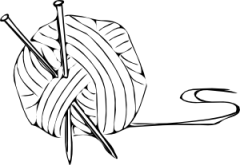
\includegraphics[width=4cm]{knit-logo}
\end{figure}
\end{column}%
\end{columns}
\end{frame}

\subsection{Overleaf}
\begin{frame}{What is Overleaf}
\begin{columns}[T] % align columns
\begin{column}{.48\textwidth}
Overleaf\footnote{\href{https://www.overleaf.com/edu/nottingham}{https://www.overleaf.com}}
\begin{itemize}
  \item Online \LaTeX editor.
  \item Collaboration features
  \item Track changes
  \item GitHub integration
  \item Basic R integration \textit{(uses only base R libraries)}
  \item Easy learning with integrated documenation
  \item It is the 'RStudio' of \LaTeX{} in my opinion
\end{itemize}
\end{column}%
\hfill%
\begin{column}{.48\textwidth}
\begin{figure}[htp]
    \centering
    
\includegraphics[width=4cm]{overleaf_wide_colour_light_bg}
\end{figure}
\end{column}%
\end{columns}
\end{frame}

\section{Code Demontrations}
\subsection{Basic Code Block}
\begin{frame}{Basic Code Block}

\begin{knitrout}
\definecolor{shadecolor}{rgb}{0.969, 0.969, 0.969}\color{fgcolor}\begin{kframe}


{\ttfamily\noindent\bfseries\color{errorcolor}{\#\# Error: <text>:7:2: unexpected symbol\\\#\# 6: \\\#\# 7: \textbackslash{}end\\\#\# \ \ \ \ \textasciicircum{}}}\end{kframe}
\end{knitrout}
